\documentclass{article}
\usepackage[pdftex]{graphicx}
\graphicspath{{../images/}}
\usepackage{boxedminipage}
\usepackage[]{ms}
%\usepackage{ms}
%\usepackage{tikz}
%\usepackage[utf8]{inputenc}

\begin{document}
\begin{titlebox}{White Dwarfs and Neutrinos}
Ilaria Caiazzo, Jeremy Heyl \\
TAs: Xianfei Zhang, Sarafina Nance, Ilka Petermann
\end{titlebox}

\section{Introduction}

The cooling of young white dwarfs is dominated by neutrinos, so young white dwarfs are a great probe of weak interactions.  In this lab, you are going to extend MESA to vary the neutrino emission rates using \texttt{run\_star\_extras} and a parameter that you can set in the \texttt{inlist}.

\section{\texttt{run\_star\_extras}}

\textbf{Task:}
\begin{enumerate}
 \setlength\itemsep{0em}
 \item 
Make a copy of your working directory from the previous lab to build your neutrino code.
\item 
You are going to replace the built-in neutrino code with your own code, so go to the directory \texttt{\$MESA\_DIR/star/other}.  You are interested in the file called \texttt{other\_neu.f90}.  Copy the subroutine \texttt{null\_other\_neu} from that file into your \texttt{run\_star\_extras.f}. You can copy it anywhere after the word \texttt{contains}, and it has to be at the same level as the other subroutines.
\item Compile MESA now by typing \texttt{./mk} in your working directory.
\item Rename the subroutine to something else, for example \texttt{my\_other\_neu}.  You do this at the top and the bottom of the subroutine.
\item 
We would like to use a parameter that we can set in the inlist (e.g.\ \texttt{s\% x\_ctrl(1)}), so we will need to define a variable \texttt{s} to hold the \texttt{star\_ptr} and then copy the \texttt{star\_ptr} into it.
\item 
The neutrino rates and their derivatives are held in the array \texttt{loss}.  You can multiply the entire array by a constant as \texttt{loss = s\% x\_ctrl(1) * loss}. This increases everything by that factor. If your new neutrino rates were more complicated than a simple multiplication, you would have to calculate the new derivatives of loss rates.
\item The array \texttt{sources} divides the loss rates by the process that generates them.  Let's multiply all of the sources by the same constant. Again, if your additional neutrinos came from a particular process, you could supply that information here.
\item
We have to let MESA know which routine to use for the new neutrino rates.  The key subroutine in \texttt{run\_star\_extras.f} is called \texttt{extras\_controls}.  It is the first subroutine in the file.  We add the command 
\begin{verbatim}
    s% other_neu => my_other_neu
\end{verbatim}
at the end of the first subroutine which tells MESA to use our routine if we ask for it.  
\item
Finally we have to tell MESA in the inlist that we want to use a new neutrino routine and the value of our control variable, so we insert the following into the controls section of the inlist
\begin{verbatim}
        use_other_neu = .true.
        x_ctrl(1) = 10
\end{verbatim}
to give ten times the neutrino cooling.
\end{enumerate}
\hint{\textbf{Solution:}\\
\\
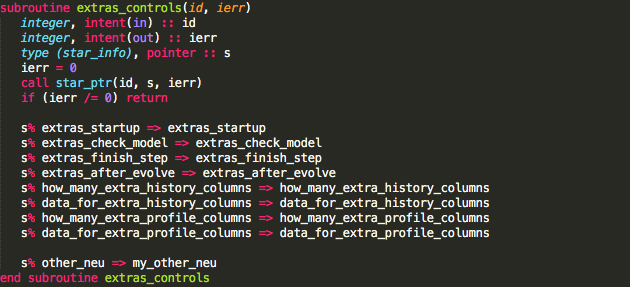
\includegraphics[width=0.8\textwidth]{extra_controls.png}

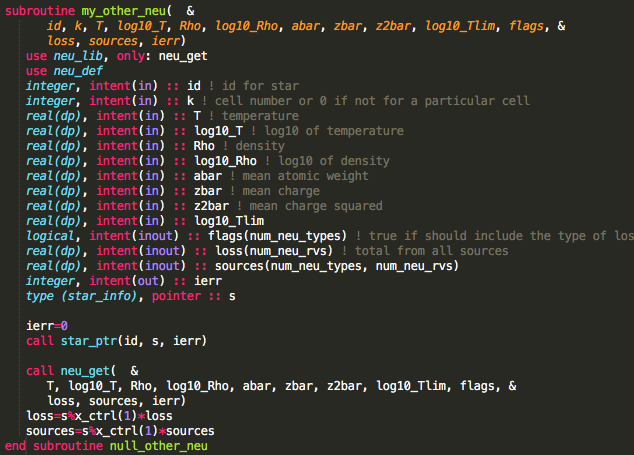
\includegraphics[width=0.8\textwidth]{my_other_neu.png}
}

\section{Evolution}

\textbf{Task:}
\begin{enumerate}
 \setlength\itemsep{0em}
    \item 
Run the evolution of the best-fitting model from the previous lab with various neutrino rates, 0.1, 0.3, 3 and 10 times the standard rate.
\item Use \texttt{paintisochone.py} to calculate the absolute magnitudes of your model white dwarfs.
\end{enumerate}

%\textbf{Bonus Task:}
%MESA keeps track of all of the various neutrino rates.  Multiply just the plasma neutrinos and add the extra neutrino %production to the totals.

\hint{\textbf{Hint:}

You may have to change the number of retries, backups and varcontrol to get the new models to work.
}

\section{Analysis}

\textbf{Task:}\vspace{-1em}
\begin{enumerate}
 \setlength\itemsep{0em}
\item Plot luminosity against effective temperature.  Does varying the neutrinos have an effect?
\item Plot luminosity against core temperature.  Does varying the neutrinos have an effect?
\item Plot luminosity against time.  Does varying the neutrinos have an effect?
 \item 
 The cumulative luminosity function measures the cooling evolution of the white dwarfs.  The young ones are bright in the ultraviolet.  Plot the cumulative luminosity functions of the observed white dwarfs in the two fields with your new models. 
 \item Remember to add the distance modulus, birth-rate estimate and possibly a shift in the age of the white dwarfs as you did in the earlier lab.
\end{enumerate}

\end{document}
